\chapter*{\textbf{Эксперимент №5: Исследование конфликтов в кэш-памяти}}
\addcontentsline{toc}{chapter}{Эксперимент №5: Исследование конфликтов в кэш-памяти}

\subsection*{\textbf{Цель эксперимента}}
Исследование влияния конфликтов кэш-памяти на эффективность вычислений.


\subsection*{\textbf{Исходные данные}}
Размер банка кэш-памяти данных первого и второго уровня, степень ассоциативности кэш-памяти первого и второго уровня, размер линейки кэш-памяти первого и второго уровня.

\subsection*{\textbf{Описание проблемы}}
Наборно-ассоциативная кэш-память состоит из линеек данных, организованных в несколько независимых банков. Выбор банка для каждой порции кэшируемых данных выполняется по ассоциативному принципу, т.е. из условия улучшения представительности выборки, в то время как целевая линейка в каждом из банков жестко определяется по младшей части физического адреса. Совокупность таких линеек всех банков принято называть набором. Таким образом, попытка читать данные из оперативной памяти с шагом, кратным размеру банка, приводит к их помещению в один и тот же набор.Если же количество запросов превосходит степень ассоциативности кэш-памяти, т.е. количество банков или количество линеек в наборе, то наблюдается постоянное вытеснение данных из кэш-памяти, причем больший ее объем остается незадействованным. 

\subsection*{\textbf{Результаты эксперимента}}
На рисунке \ref{img:experiment_5} представлен график, полученный в результате эксперимента с исходными параметрами:
\begin{itemize}
	\item Размер банка кэш-памяти (К) = 128;
	\item Размер линейки кэш-памяти (б) = 128;
	\item Количество читаемых линеек = 32.
\end{itemize}

\begin{figure}[H]
	\centering{
		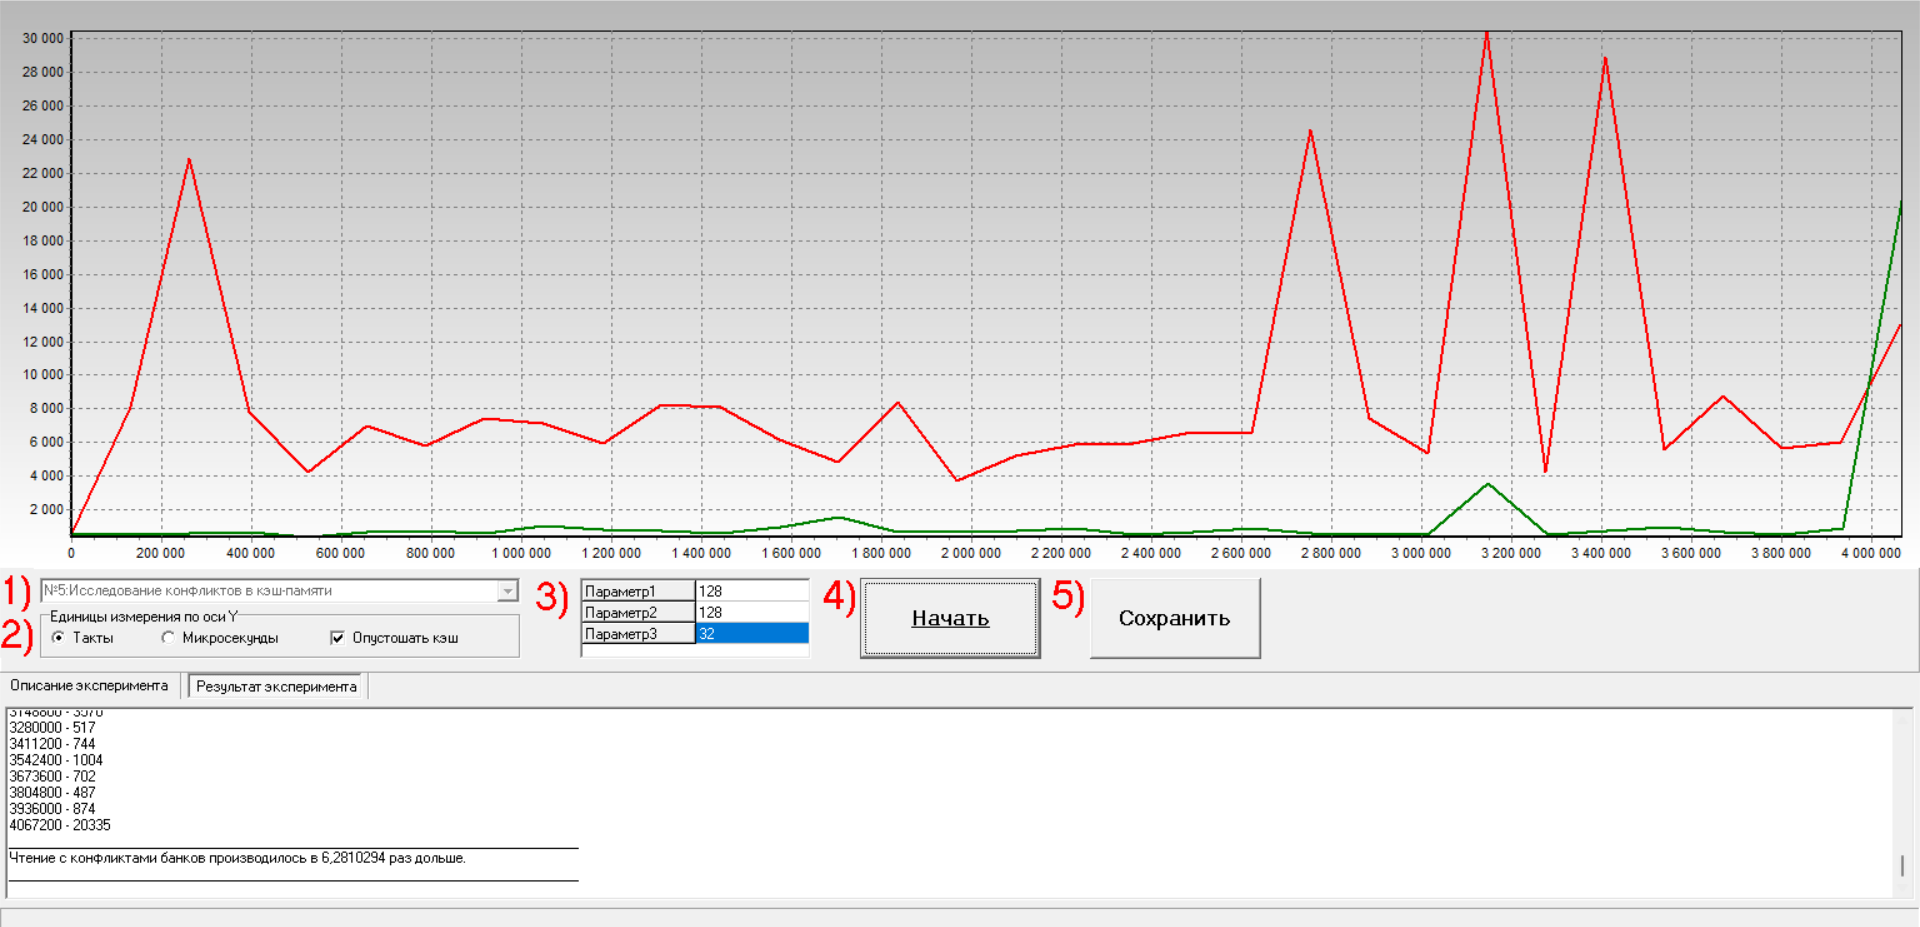
\includegraphics[scale=0.4]{images/experiment_5_1}
		\caption{Эксперимент №5}
		\label{img:experiment_5}
	}
\end{figure}

Результат сравнения времени (как вывод программы) представлен на рисунке \ref{img:experiment_5}. Как видно на рисунке, чтение с конфликтами банков производилось в 3,68 раз дольше.

Красный график показывает время или количество тактов работы процедуры, читающей данные с конфликтами в кэш-памяти. 

Зеленый график показывает время или количество тактов работы процедуры, не вызывающей конфликтов в кэш-памяти. Ось абсцисс отражает смещение читаемой ячейки от начала блока данных.

Красный график соответствует алгоритму, который построен таким образом, что чтение данных выполняется с шагом, кратным размеру банка. Именно это и порождает постоянные конфликты в кэш-памяти.

Зеленый график соответствует алгоритму, который оптимизируется размещение данных в кэш с помощью задания смещения востребованных данных на шаг, достаточный для выбора другого набора. (Шаг соответствует размеру линейки).

\subsection*{Вывод}
Использование кэш-памяти работа процессора ускоряется в 3,68 раз.